% ********************************************************************
% *                  Format for IMVIP 2019  papers,                  *
% *         based on the IMVIP 2001, 2006, 2014-2018 templates       *
% ********************************************************************
\documentclass[a4paper,11pt]{article}



\setlength{\topmargin}{-0.5cm}
\setlength{\headsep}{.5cm}
%\setlength{\footskip}{1.0cm}
\setlength{\textheight}{24cm}
\setlength{\textwidth}{17cm}
\setlength{\evensidemargin}{-.5cm}
\setlength{\oddsidemargin}{-.5cm}



\usepackage{fourier}
\usepackage{color}
 \usepackage{graphicx}
\usepackage{url}
\usepackage[affil-it]{authblk}
\usepackage{amsmath}
\usepackage{wrapfig}
\usepackage{xspace}

\usepackage[T1]{fontenc}
\usepackage{times}

\usepackage{booktabs}

\usepackage{cite}

\pagestyle{empty}

%%%%
\begin{document}

\title{Machine Learning (09012) Individual Assignment 2020}

\author{Mark Breen}
\affil{Insitute of Technology, Sligo}
\date{}
\maketitle
\thispagestyle{empty}



\begin{abstract}
Object classification systems utilised in autonomous vehicles must be fast, accurate and scalable. Transfer learning is a machine learning technique where a model trained on one dataset is re-used for predictions on a different dataset. In this paper, a VGG16 model will be re-trained on the German Traffic Sign Benchmark (GTSRB). For comparison purposes, a number of different models will be evaluated, each originating from the VGG16 network but with different layers frozen. The accuracy and training time for each of the four models will be discussed.
\end{abstract}
\textbf{Keywords:} Transfer Learning, VGG16, Machine Vision, Autonomous Vehicles



%%%%%%%%%%%%%%%%%%%%%%
\section{Introduction}

%%%%%%%%%%%%%%%%%%%%%%
Object classification plays a key role in making Advanced Driver Assistance Systems (ADAS) accurate, reliable and safe. One such application of object classification in the context of autonomous vehicles is the ability to detect and classify road signs in images. Classification of road signs is of vital importance when an autonomous vehicle is driving since they can be used to tell the vehicle what speed to travel at, alert vehicles that a stop sign is expected, whether to yield, and alert the vehicle of potentially dangerous zones such as schools, for example.

In traditional Machine Learning approaches, the pipeline typically involves gathering a large amount of data, fitting a model to that data and performing validation. In the context of image classification problems, where typically the data is very high dimensional, an enormous number of parameters may be required to be optimised. 

Transfer learning is an approach to machine learning problems whereby a model trained on one dataset is re-used for predictions on a different task. Transfer learning can be very useful since the entire network does not need to be retrained. This saves resources and time, while still maintaining the inferential quality and well-trained feature exatraction abilities of a larger network. The network that will be utilised in this paper is the VGG16 network.

%%

\section{Methods}

This section will describe the data utilised along with the model training and validation process. All work was done using Python version 3.8.5 and TensorFlow 2.4.0. Training was done using an Nvidia RTX 3070 Graphics Processing Unit

\subsection{Hardware}

All work was done on a PC with an Intel 6-core processor, 16 Gigabytes of RAM and an Nvidia RTX 3070 Graphics Processing Unit (GPU)

\subsection{Software}

All work was done using Python 3.8.5. TensorFlow 2.4.0 was using to load, train and test the VGG16 model.

\subsection{Data}

The German Traffic Sign Benchmark (GTSRB) will be used in this paper. This dataset contains images of road traffic signs in Germany. The training dataset contains 43 classes of images, and more than 50,000 images in total. 

The images will be resized to a height of 48 pixels and width of 48 pixels in order to reduce the strain on the system memory and GPU. It is hoped that the image size of 48x48 will be sufficient resolution for the GTSRB images since the actual images in the database are not complex.

The images are stored as tensors of dimension $(48, 48, 3)$. Since the images are colour, each pixel has corresponding Red, Green and Blue values. These three values have a range of $0-255$. The input images will be normalised by dividing the RGB input values by $255$ to ensure that all input values instead have a range of $0-1$.

The training data will be split into a training and validation set. The training dataset will contain $80\%$ of the training data, and the validation set will comprise of the remaining $20\%$ of the data.

The testing dataset will be reserved until all model training and tuning has been completed.


\subsection{VGG16}

In a study which aimed to explore the effect of the convolutional neural network depth on its accuracy \cite{Simonyan2015}, two networks were used in a submission to the ImageNet Challenge in 2014 which achieved first and second place. These networks, commonly referred to as VGG16 and VGG19 were made publically available for use. 

For this paper, the three full-connected layers at the top of the network will not be included. This allows the input size to be defined. A custom dense layer will be added to the network to make it capable of identifying the 43 classes of roadsign that are relevant to this dataset, rather than the 1000 image classes that exist in the ImageNet dataset. Since the convolution layers are what work as the feature extractors, it is hoped that the network will do a good job when retrained to the GTSRB dataset. The architecure of this adapted VGG16 network is shown in Figure \ref{fig:myfig}. 

\begin{figure}[!ht]
	\begin{center}
		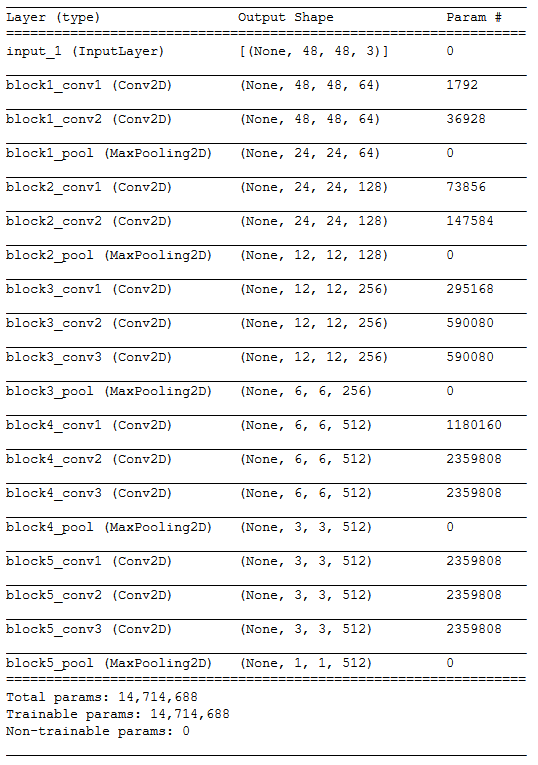
\includegraphics[width=0.5\textwidth]{network_architecture.png}
	\end{center}
	\vspace{-20pt}
	\caption{VGG16 Network Architecture}\label{fig:myfig}
	\vspace{-10pt}
\end{figure}

\subsection{Model Training}

The adapted VGG16 network is trained for $20$ epochs, using a batch size of $256$. The Categorical Crossentropy loss function will be used, along with an accuracy metric.

A number of different models will be fitted fitted. 

\subsubsection{VGG16\_1}

In order to get a baseline estimate of how the VGG16 weights transfer to the GTSRB dataset, initially all layers in the VGG16 model will be frozen, so only the final dense layer will be retrained in order to adapt the model to the $43$ classes contained in the GTSRB database.

\subsubsection{VGG16\_2}

This model will have all layers before the block 5 convolutional layers frozen.

\subsubsection{VGG16\_3}

This model will have all layers before the block 4 convolutional layers frozen.

\subsubsection{VGG16\_4}

This model will have no layers frozen, i.e. it will be completely retrained. Although this isn't necessarily in the scope of this paper it is still of interest to see how the architecture of the VGG16 network performs when utilised in a different classification problem. It is expected that this model will perform the best, thus the main purpose of it's inclusion is to compare the tradeoff between the accuracy gain of adding additional training layers and the computational expense incurred in doing so.

\subsection{Model Validation}	

The accuracy of the model will be computed in order to assess performance. The accuracy is the number of correct classifications divided by the number of samples in the dataset.

\section{Results}

The accuracy scores for each model evaluated on the test set is shown in Table \ref{tab:model_accuracy}. As can be seen in this table, the baseline VGG16\_1 model achieves an accuracy score of $61.89\%$. The model is trained in a relative fast time of $98.72s$. For the amount of training time invested, this is a good start. 

VGG16\_2, the model where the convolutional layers are re-trained using the GTSRB dataset, however, shows a significant increase in performance over the VGG16\_1 model. The VGG16\_2 model achieves an accuracy score of $80.84\%$ and is trained in $113.67s$.

VGG16\_3 and VGG16\_4 achieve very good accuracy scores of $93.55\%$ and $96.83\%$, respectively. The training times, however, are also significantly larger than the baseline VGG16\_1 model, especially the VGG16\_4 model. This, however, is as expected since the more parameters that are required to be optimised the greater the training time.

% Please add the following required packages to your document preamble:
% \usepackage{booktabs}
\begin{table}[]
	\begin{center}
	\begin{tabular}{@{}llll@{}}
		\toprule
		Model    & Loss   & Accuracy (\%) & Training Time (s) \\ \midrule
		VGG16\_1 & 2.0551 & 61.89         & 98.72             \\
		VGG16\_2 & 1.2842 & 80.84         & 113.67            \\
		VGG16\_3 & 0.3379 & 93.55         & 155.15            \\
		VGG16\_4 & 0.1597 & 96.83         & 248.09            \\ \bottomrule
	\end{tabular}
	\end{center}
\vspace{-20pt}
\caption{Accuracy, loss and training time for four different models.} \label{tab:model_accuracy}
\vspace{-10pt}
\end{table}

\section{Conclusions}

Since there are $43$ classes in the image dataset, this means that the probability of randomly selecting the correct class for any given image is $2.3\%$. The baseline VGG16\_1 model evidently performs significantly better than this with an accuracy score of $61.89\%$. Given that the goal of this paper is to create a classification model intended to be used in an autonomous vehicle, however, clearly a higher accuracy is required. Since the safety of the vehicle passengers, along with other road users is of the upmost importance, this means that an autonomous vehicle needs to have the ability to detect and classify it's surroundings to a very high degree of accuracy. If, for example, a $20km/h$ was identified as a $60km/h$ speed sign this could result in an autonomous vehicle driving at three times the speed limit which is incredibly dangerous both for passengers and other road users.

Similarly, if the vehicle fails to identify a stop sign, it could result in the vehicle not stopping at a required spot, potentially causing an accident. The level of accuracy obtained by the baseline model, in this context, is deemed to be not accurate enough. The problem is that while some of the feature extraction ability of the network is transferred over to the new dataset, it could be the case that the road signs are too closely related to one another and the original VGG16 network simply would not have been exposed to this type of image before. 

Thankfully, performance is greatly enhanced by retraining additional layers of the network. When the fifth convolutional block of the VGG16 network is retrained, accuracy increases by almost $20\%$, resulting in an accuracy level of $80.84\%$. This increase is promising, especially since the training time only increases by $15\%$. When the fourth and fifth convolutional block is retrained, the accuracy increases to $93.55\%$, with a percentage increase in training time over the baseline VGG16\_1 model of $57\%$. For the sake of completeness, all layers of the VGG16 network were also retrained, yielding an accuracy of $96.83\%$, however the training time over the baseline VGG16\_1 model more than doubled.

Taking the training time into account, the accuracy obtained by training the fourth and fifth layers in model VGG16\_3 appears to be the best in terms of the tradeoff between accuracy and computing power required for training. This network has done an excellent job at extracting features from the GTSRB dataset while still maintaining most of the architecture and weights of the original VGG16 network. 

Further work in this area might involve expanding the road signs to other european countries, along with creating a bootstrapped image dataset by randomly sampling images and performing small transformations such as rotations. It is hoped that in further work, the creation of more samples would help the network extract more features from the data.


\bibliographystyle{IEEEtran}
\typeout{}
\bibliography{IEEEabrv, ml_individual.bib}


\end{document}

